%%%% Proceedings format for most of ACM conferences (with the exceptions listed below) and all ICPS volumes.
\documentclass[sigconf]{acmart}
\usepackage{graphicx}
\graphicspath{{imgs/}}
\usepackage[english,ngerman,brazilian]{babel}
\settopmatter{printacmref=false}
\setcopyright{none}
\renewcommand\footnotetextcopyrightpermission[1]{}
\pagestyle{plain}

\def\BibTeX{{\rm B\kern-.05em{\sc i\kern-.025em b}\kern-.08emT\kern-.1667em\lower.7ex\hbox{E}\kern-.125emX}}

% end of the preamble, start of the body of the document source.
\begin{document}

%
% The "title" command has an optional parameter, allowing the author to define a "short title" to be used in page headers.
\title[Fronteiras da Transferência de Aprendizagem: uma revisão sistemática com enfoque meta-analítico]{Fronteiras da Transferência de Aprendizagem: \\
uma revisão sistemática com enfoque meta-analítico}
%
% The "author" command and its associated commands are used to define the authors and their affiliations.
% Of note is the shared affiliation of the first two authors, and the "authornote" and "authornotemark" commands
% used to denote shared contribution to the research.
\author{Fred Guth}
% \authornote{Both authors contributed equally to this research.}
\email{fredguth@fredguth.com}
\affiliation{%
  \institution{Departamento de Ciência de Computação, Universidade de Brasília}
  \postcode{70.910-900}
  \city{Brasília}
  \state{DF}
  \country{Brazil}
}

%
% By default, the full list of authors will be used in the page headers. Often, this list is too long, and will overlap
% other information printed in the page headers. This command allows the author to define a more concise list
% of authors' names for this purpose.
\renewcommand{\shortauthors}{Guth,.}

%
% The abstract is a short summary of the work to be presented in the article.
\begin{abstract}
A clear and well-documented \LaTeX\ document is presented as an article formatted for publication by ACM in 
a conference proceedings or journal publication. Based on the ``acmart'' document class, this article presents
and explains many of the common variations, as well as many of the formatting elements
an author may use in the preparation of the documentation of their work.
\end{abstract}

%
% The code below is generated by the tool at http://dl.acm.org/ccs.cfm.
% Please copy and paste the code instead of the example below.
%

\begin{CCSXML}
<ccs2012>
 <concept>
 <concept_id>10010147.10010257.10010258.10010262.10010277</concept_id>
 <concept_desc>Computing methodologies~Transfer learning</concept_desc>
 <concept_significance>500</concept_significance>
 </concept>
</ccs2012>
\end{CCSXML}

\ccsdesc[500]{Computing methodologies~Transfer learning}


%
% Keywords. The author(s) should pick words that accurately describe the work being
% presented. Separate the keywords with commas.

\keywords{transferência de aprendizado, revisão sistemática, enfoque meta-analítico}

%
% A "teaser" image appears between the author and affiliation information and the body 
% of the document, and typically spans the page. 
% \begin{teaserfigure}
%   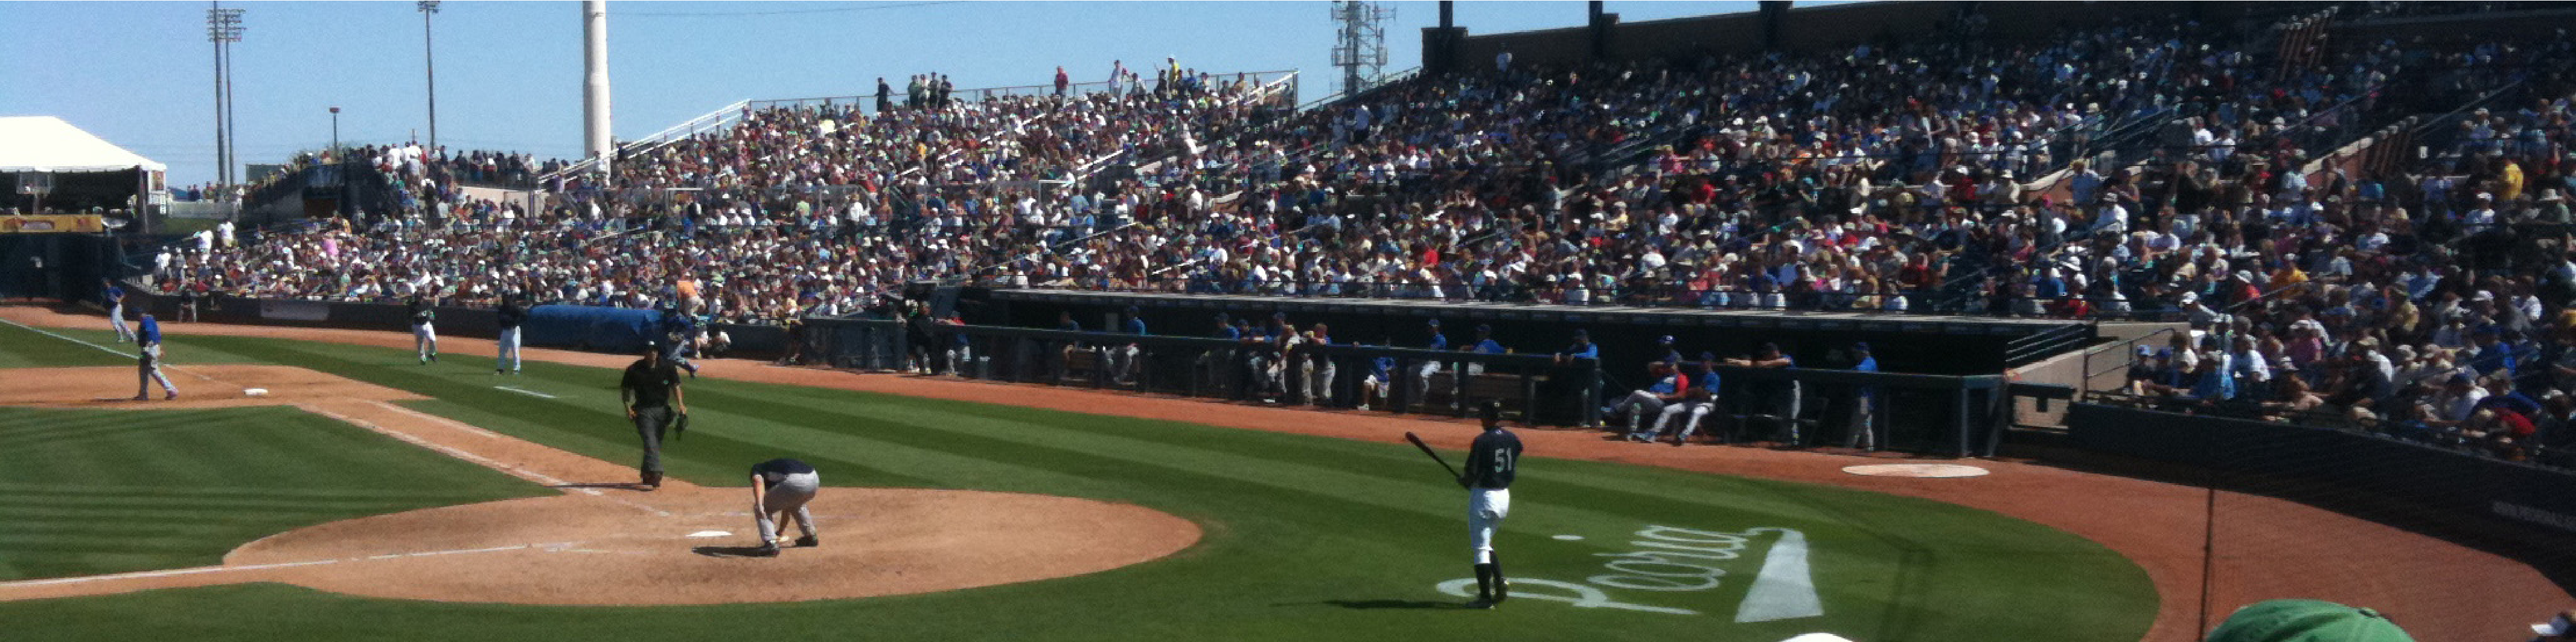
\includegraphics[width=\textwidth]{sampleteaser}
%   \caption{Seattle Mariners at Spring Training, 2010.}
%   \Description{Enjoying the baseball game from the third-base seats. Ichiro Suzuki preparing to bat.}
%   \label{fig:teaser}
% \end{teaserfigure}

%
% This command processes the author and affiliation and title information and builds
% the first part of the formatted document.
\maketitle

\section{Introdução} 
  \subsection{Contribuições}
  \subsection{Visão Geral e Organização do Artigo}
  \subsection{Trabalhos Relacionados}
\section{Método de Revisão Sistemática}
  \subsection{O Enfoque Meta Analítico}
  \subsection{Análise de Co-citações}
  \subsection{Análise de Acoplamento Bibliográfico}
  \subsection{Análise Textual}
  \subsection{Sumarização}
\subsection{Revisão da Literatura}
  \subsection{Transferência de Aprendizagem}
  \subsection{Um breve histórico}
  \subsection{Os Clássicos}
  \subsection{A Fronteira}
\section{Problemas em Aberto}
\section{Conclusão}

\section{Citations and Bibliographies}

The use of \BibTeX\ for the preparation and formatting of one's references is strongly recommended. Authors' names should be complete --- use full first names (``Donald E. Knuth'') not initials (``D. E. Knuth'') --- and the salient identifying features of a reference should be included: title, year, volume, number, pages, article DOI, etc. 

The bibliography is included in your source document with these two commands, placed just before the \verb|\end{document}| command:
\begin{verbatim}
  \bibliographystyle{ACM-Reference-Format}
  \bibliography{bibfile}
\end{verbatim}
where ``\verb|bibfile|'' is the name, without the ``\verb|.bib|'' suffix, of the \BibTeX\ file.

Citations and references are numbered by default. A small number of ACM publications have citations and references formatted in the ``author year'' style; for these exceptions, please include this command in the {\bf preamble} (before ``\verb|\begin{document}|'') of your \LaTeX\ source: 
\begin{verbatim}
  \citestyle{acmauthoryear}
\end{verbatim}

Some examples.  A paginated journal article \cite{Abril07}, an enumerated journal article \cite{Cohen07}, a reference to an entire issue \cite{JCohen96}, a monograph (whole book) \cite{Kosiur01}, a monograph/whole book in a series (see 2a in spec. document)
\cite{Harel79}, a divisible-book such as an anthology or compilation \cite{Editor00} followed by the same example, however we only output the series if the volume number is given \cite{Editor00a} (so Editor00a's series should NOT be present since it has no vol. no.),
a chapter in a divisible book \cite{Spector90}, a chapter in a divisible book in a series \cite{Douglass98}, a multi-volume work as book \cite{Knuth97}, an article in a proceedings (of a conference, symposium, workshop for example) (paginated proceedings article) \cite{Andler79}, a proceedings article with all possible elements \cite{Smith10}, an example of an enumerated proceedings article \cite{VanGundy07}, an informally published work \cite{Harel78}, a doctoral dissertation \cite{Clarkson85}, a master's thesis: \cite{anisi03}, an online document / world wide web resource \cite{Thornburg01, Ablamowicz07, Poker06}, a video game (Case 1) \cite{Obama08} and (Case 2) \cite{Novak03} and \cite{Lee05} and (Case 3) a patent \cite{JoeScientist001}, work accepted for publication \cite{rous08}, 'YYYYb'-test for prolific author \cite{SaeediMEJ10} and \cite{SaeediJETC10}. Other cites might contain 'duplicate' DOI and URLs (some SIAM articles) \cite{Kirschmer:2010:AEI:1958016.1958018}. Boris / Barbara Beeton: multi-volume works as books \cite{MR781536} and \cite{MR781537}. A couple of citations with DOIs: \cite{2004:ITE:1009386.1010128,Kirschmer:2010:AEI:1958016.1958018}. Online citations: \cite{TUGInstmem, Thornburg01, CTANacmart}.


\bibliographystyle{ACM-Reference-Format}
\bibliography{reference}



\end{document}
